\chapter{Bottom-Up Parsing}

\section{Idea}

A \textbf{bottom-up} parser builds the tree from the leaves up. It reads tokens onto a stack
(\textbf{shift}) and, when the top of the stack matches the right-hand side of a production,
replaces it with the left-hand side (\textbf{reduce}). Read in reverse, the reductions form a
\emph{rightmost derivation}. Such parsers are called \textbf{LR}: \textbf{L}eft-to-right scan,
\textbf{R}ightmost derivation in reverse.

Invariant: \emph{stack (bottom to top)} $+$ \emph{unread input} $=$ a sentential form of the
rightmost derivation.

\begin{example}
Grammar: $S'\to\ \vdash E\dashv$, $E\to E+T \mid T$, $T\to\mathtt{id}$.
\begin{center}
\small
\begin{tabular}{lll}
\toprule
stack & input & action \\
\midrule
 & $\vdash$ id + id $\dashv$ & shift \\
$\vdash$ & id + id $\dashv$ & shift \\
$\vdash$ id & + id $\dashv$ & reduce $T\to$ id \\
$\vdash T$ & + id $\dashv$ & reduce $E\to T$ \\
$\vdash E$ & + id $\dashv$ & shift \\
$\vdash E +$ & id $\dashv$ & shift \\
$\vdash E +$ id & $\dashv$ & reduce $T\to$ id \\
$\vdash E + T$ & $\dashv$ & reduce $E \to E+T$ \\
$\vdash E$ & $\dashv$ & shift \\
$\vdash E \dashv$ & & reduce $S' \to\ \vdash E\dashv$, accept \\
\bottomrule
\end{tabular}
\end{center}
\end{example}

Each reduction creates one interior node of the parse tree, from the leaves upward. Numbering
the nodes in the order the reductions happen:
\begin{center}
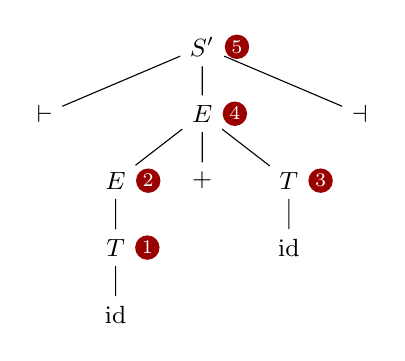
\begin{tikzpicture}[level distance=0.85cm,every node/.style={font=\small},
  level 1/.style={sibling distance=2cm},level 2/.style={sibling distance=1.1cm},
  num/.style={label={[font=\scriptsize,text=white,fill=red!60!black,circle,inner sep=1pt]right:#1}}]
\node[num=5] {$S'$}
  child {node {$\vdash$}}
  child {node[num=4] {$E$}
    child {node[num=2] {$E$} child {node[num=1] {$T$} child {node {id}}}}
    child {node {$+$}}
    child {node[num=3] {$T$} child {node {id}}}}
  child {node {$\dashv$}};
\end{tikzpicture}
\end{center}
Reading the reductions backwards (5, 4, 3, 2, 1) expands the rightmost non-terminal each time.

The hard question is \emph{when} to shift and when to reduce (and by which rule). Note that
the stack in the third row could be reduced in many ways; we must only reduce when the result
can still be extended to a valid parse.

\section{Viable prefixes and items}

\begin{definition}
A \textbf{viable prefix} is a prefix of a right sentential form that does not extend past the
right end of the next handle to be reduced. The stack of a correct LR parser always holds a
viable prefix.
\end{definition}

\begin{theorem}[Knuth, 1965]
For any CFG, the set of viable prefixes is a \emph{regular language}.
\end{theorem}

So a DFA can read the stack and tell us what to do. Its states are built from items.

\begin{definition}
An \textbf{LR(0) item} is a production with a dot somewhere in its right-hand side, e.g.\
$E\to E\,\bullet + T$. The dot marks how much of the RHS is already on the stack. An item
with the dot at the end, $A\to\alpha\bullet$, is a \textbf{complete} (reduce) item.
\end{definition}

\section{Building the LR(0) automaton}

\begin{enumerate}
  \item Start state: the \textbf{closure} of $\{S' \to \bullet \vdash S\dashv\}$.
  \item \textbf{Closure}: whenever a state contains $A \to \alpha\bullet B\beta$ with $B$ a
        non-terminal, add $B \to \bullet\gamma$ for every production of $B$; repeat.
  \item \textbf{Goto}: from state $I$ on symbol $X$, take every item $A\to\alpha\bullet X\beta$
        in $I$, move the dot over $X$ to get $A\to\alpha X\bullet\beta$, and take the closure.
  \item Repeat until no new states appear.
\end{enumerate}

\begin{example}[LR(0) automaton for $S'\to\ \vdash E\dashv$, $E\to E+T\mid T$, $T\to\mathtt{id}$]
States are boxes listing their items; edges are goto transitions.
\begin{center}
\begin{tikzpicture}[>=Stealth, st/.style={draw,rectangle,rounded corners,align=left,font=\scriptsize,inner sep=3pt}]
  \node[st] (0) at (0,0) {\textbf{0}\\ $S'\to\bullet\vdash E\dashv$};
  \node[st] (1) at (3.4,0) {\textbf{1}\\ $S'\to\ \vdash\bullet E\dashv$\\ $E\to\bullet E+T$\\ $E\to\bullet T$\\ $T\to\bullet\mathtt{id}$};
  \node[st] (2) at (7.2,0) {\textbf{2}\\ $S'\to\ \vdash E\bullet\dashv$\\ $E\to E\bullet+T$};
  \node[st] (5) at (10.6,0) {\textbf{5}\\ $S'\to\ \vdash E\dashv\bullet$};
  \node[st] (3) at (3.4,-2.6) {\textbf{3}\\ $E\to T\bullet$};
  \node[st] (4) at (7.2,-4.2) {\textbf{4}\\ $T\to\mathtt{id}\bullet$};
  \node[st] (6) at (7.2,-2.2) {\textbf{6}\\ $E\to E+\bullet T$\\ $T\to\bullet\mathtt{id}$};
  \node[st] (7) at (10.6,-2.2) {\textbf{7}\\ $E\to E+T\bullet$};
  \draw[->] (-1.3,0) -- (0);
  \draw[->] (0) -- node[above,font=\scriptsize]{$\vdash$} (1);
  \draw[->] (1) -- node[above,font=\scriptsize]{$E$} (2);
  \draw[->] (2) -- node[above,font=\scriptsize]{$\dashv$} (5);
  \draw[->] (1) -- node[left,font=\scriptsize]{$T$} (3);
  \draw[->] (1.south east) to[out=-60,in=180] node[below,font=\scriptsize]{id} (4);
  \draw[->] (2) -- node[left,font=\scriptsize]{$+$} (6);
  \draw[->] (6) -- node[above,font=\scriptsize]{$T$} (7);
  \draw[->] (6) -- node[left,font=\scriptsize]{id} (4);
\end{tikzpicture}
\end{center}
States 3, 4, 5, 7 contain one complete item and nothing else: reduce states.
\end{example}

\section{The LR parsing algorithm}

Rather than re-running the DFA over the whole stack after every reduction, keep a stack of
DFA \emph{states} alongside the symbols.

\begin{lstlisting}[style=cpp]
stateStack.push(start);
for each token a (BOF, ..., EOF):
    // reduce as long as the current state says so
    while (Reduce[top(stateStack)][a] == A -> gamma) {
        output "A -> gamma";
        pop |gamma| symbols and states;
        push A; stateStack.push(Goto[top(stateStack)][A]);
    }
    if (Shift[top(stateStack)][a] is undefined) reject (error at token a);
    push a; stateStack.push(Shift[top(stateStack)][a]);
accept (after shifting EOF, reduce by S' -> BOF S EOF)
\end{lstlisting}

Each reduction costs $\bigO(|\gamma|)$ and every token is shifted once, so the parser runs in
$\bigO(n)$ time for a grammar of fixed size. The output, a list of productions, is a reverse
rightmost derivation; the CS 241 WLP4 parser prints it reversed (as a preorder traversal,
i.e.\ a leftmost derivation) by building the tree on the fly.

\begin{example}[Trace with states]
Parsing $\vdash \mathtt{id}+\mathtt{id}\dashv$ with the automaton above:
\begin{center}
\small
\begin{tabular}{lll}
\toprule
state stack & input & action \\
\midrule
0 & $\vdash$ id + id $\dashv$ & shift $\to$ 1 \\
0 1 & id + id $\dashv$ & shift $\to$ 4 \\
0 1 4 & + id $\dashv$ & reduce $T\to$id; Goto(1,$T$)=3 \\
0 1 3 & + id $\dashv$ & reduce $E\to T$; Goto(1,$E$)=2 \\
0 1 2 & + id $\dashv$ & shift $\to$ 6 \\
0 1 2 6 & id $\dashv$ & shift $\to$ 4 \\
0 1 2 6 4 & $\dashv$ & reduce $T\to$id; Goto(6,$T$)=7 \\
0 1 2 6 7 & $\dashv$ & reduce $E\to E+T$ (pop 3); Goto(1,$E$)=2 \\
0 1 2 & $\dashv$ & shift $\to$ 5; accept \\
\bottomrule
\end{tabular}
\end{center}
\end{example}

\section{Conflicts}

A state is problematic if it has
\begin{itemize}
  \item a \textbf{shift-reduce conflict}: a complete item $A\to\alpha\bullet$ and an item
        $B\to\beta\bullet a\gamma$ (could shift $a$ or reduce), or
  \item a \textbf{reduce-reduce conflict}: two complete items $A\to\alpha\bullet$ and
        $B\to\beta\bullet$.
\end{itemize}
A grammar is \textbf{LR(0)} iff its LR(0) automaton has no conflicts: then every reduce
state can reduce without looking at the next token.

\begin{example}[LR(0) fails]
Make $+$ right-associative: $E \to T + E \mid T$, $T\to\mathtt{id}$. After reading $T$ the
state contains
\[
E \to T\bullet + E \qquad\text{and}\qquad E\to T\bullet
\]
a shift-reduce conflict: should we reduce $T$ to $E$, or shift the $+$?
\end{example}
\begin{center}
\begin{tikzpicture}[>=Stealth, st/.style={draw,rectangle,rounded corners,align=left,font=\scriptsize,inner sep=3pt}]
  \node[st] (1) at (0,0) {$S'\to\ \vdash\bullet E\dashv$\\ $E\to\bullet T+E$\\ $E\to\bullet T$\\ $T\to\bullet\mathtt{id}$};
  \node[st,draw=red!70!black,very thick] (c) at (4,0) {$E\to T\bullet + E$\\ $E\to T\bullet$};
  \node[st] (n) at (8,0) {$E\to T+\bullet E$\\ $E\to\bullet T+E$\\ $E\to\bullet T$\\ $T\to\bullet\mathtt{id}$};
  \draw[->] (1) -- node[above,font=\scriptsize]{$T$} (c);
  \draw[->] (c) -- node[above,font=\scriptsize]{$+$} (n);
  \node[font=\scriptsize,red!70!black,align=center,below=3pt of c] {shift $+$ \emph{or}\\ reduce $E\to T$?};
\end{tikzpicture}
\end{center}

\section{SLR(1)}

\textbf{Simple LR(1)} uses the same LR(0) automaton, but only reduces by $A\to\alpha\bullet$
when the lookahead is in $\mathrm{Follow}(A)$.

In the example above, $\mathrm{Follow}(E) = \{\dashv\}$, so in that state: on $+$ shift, on
$\dashv$ reduce $E\to T$. The conflict is gone. A grammar is SLR(1) iff for every state:
the Follow sets of its complete items are pairwise disjoint and disjoint from the terminals
that can be shifted.

\section{LR(1) and LALR(1)}

Follow sets are global: $\mathrm{Follow}(A)$ includes everything that can follow $A$
\emph{anywhere}, which may be too coarse in a particular state. LR(1) refines the items.

\begin{definition}
An \textbf{LR(1) item} $[A\to\alpha\bullet\beta,\ a]$ pairs an LR(0) item with a lookahead
terminal $a$, meaning ``we are in the middle of $A\to\alpha\beta$, and after it the input
should continue with $a$''. Closure: for $[A\to\alpha\bullet B\beta,\ a]$ add
$[B\to\bullet\gamma,\ b]$ for every $b \in \mathrm{First}(\beta a)$. Reduce by
$[A\to\alpha\bullet,\ a]$ only when the lookahead is $a$.
\end{definition}

LR(1) is very powerful: almost all programming-language grammars are LR(1), and LR(1)
grammars describe exactly the deterministic context-free languages. But LR(1) automata can
have many more states than LR(0) (several copies of a state differing only in lookaheads).

\textbf{LALR(1)} (look-ahead LR) merges LR(1) states with identical \emph{cores} (the same
LR(0) items), unioning their lookaheads. The result has the same number of states as the
LR(0) automaton but more precise lookaheads than SLR. Merging cannot introduce new
shift-reduce conflicts but can introduce reduce-reduce conflicts.

\begin{example}[LR(1) but not LALR(1)]
$S \to a A d \mid b B d \mid a B e \mid b A e$, $A \to c$, $B\to c$. After $a\,c$ the LR(1)
state is $\{[A\to c\bullet, d], [B\to c\bullet, e]\}$; after $b\,c$ it is
$\{[A\to c\bullet, e], [B\to c\bullet, d]\}$. Both have the same core, so LALR merges them into
$\{[A\to c\bullet, d/e], [B\to c\bullet, d/e]\}$: a reduce-reduce conflict.
\end{example}
\begin{center}
\begin{tikzpicture}[>=Stealth, st/.style={draw,rectangle,rounded corners,align=left,font=\scriptsize,inner sep=3pt}]
  \node[st] (a) at (0,0.9) {after $a\,c$:\\ $[A\to c\bullet,\ d]$\\ $[B\to c\bullet,\ e]$};
  \node[st] (b) at (0,-0.9) {after $b\,c$:\\ $[A\to c\bullet,\ e]$\\ $[B\to c\bullet,\ d]$};
  \node[st,draw=red!70!black,very thick] (m) at (5,0) {LALR merge:\\ $[A\to c\bullet,\ d/e]$\\ $[B\to c\bullet,\ d/e]$};
  \draw[->] (a.east) -- (m.west);
  \draw[->] (b.east) -- (m.west);
  \node[font=\scriptsize,align=center] at (0,-2.0) {LR(1): each state reduces\\ by a different rule on $d$ and on $e$};
  \node[font=\scriptsize,red!70!black,align=center,below=3pt of m] {on $d$ (and on $e$):\\ reduce by $A\to c$ or $B\to c$?};
\end{tikzpicture}
\end{center}

\begin{center}
\begin{tabular}{lll}
\toprule
method & automaton & reduce $A\to\alpha\bullet$ when lookahead is in \\
\midrule
LR(0) & LR(0) items & (always) \\
SLR(1) & LR(0) items & $\mathrm{Follow}(A)$ \\
LALR(1) & LR(0) cores, merged LR(1) lookaheads & state-specific lookahead set \\
LR(1) & LR(1) items & item's own lookahead \\
\bottomrule
\end{tabular}
\end{center}
Strength: LR(0) $\subset$ SLR(1) $\subset$ LALR(1) $\subset$ LR(1) (as grammar classes).
Tools such as yacc and bison generate LALR(1) parsers. Every LL(1) grammar is LR(1), but
not vice versa; in particular LR parsers handle left recursion naturally (and in fact
prefer it, since it keeps the stack shallow).

\section{Parsing WLP4}

In the assignments, the WLP4 grammar's LR(1) DFA (transitions and reductions) was provided
in a file; we implemented the driver loop above and output the parse tree. Error reporting:
when no shift is possible, report the position of the offending token.

\section{Summary}
\begin{itemize}
  \item Shift tokens; reduce when the stack top is a handle. Reductions give a rightmost derivation in reverse.
  \item The viable prefixes form a regular language, recognised by the LR(0) item automaton (closure + goto).
  \item Keep a stack of states so each step is $\bigO(1)$ amortised; overall linear time.
  \item Conflicts: shift-reduce and reduce-reduce. LR(0) allows none.
  \item SLR(1) uses Follow sets; LR(1) attaches lookaheads to items; LALR(1) merges LR(1)
        states with equal cores (may create reduce-reduce conflicts).
\end{itemize}
